\documentclass[a4paper,14pt]{article}

\usepackage{cmap}					
\usepackage[T2A]{fontenc}			
\usepackage[utf8]{inputenc}			
\usepackage[english,russian]{babel}	

\usepackage{amsmath,amsfonts,amssymb,amsthm,mathtools} 
\usepackage{wasysym}


\usepackage{tikz}
\usepackage{filecontents}
\usetikzlibrary{datavisualization}
\usetikzlibrary{datavisualization.formats.functions}
\usepackage{graphicx}
\usepackage{listings}
\usepackage{color}
\usepackage{amsmath}
\usepackage{pgfplots}
\usepackage{url}

\usepackage{indentfirst}
\usepackage{amssymb}


\usepackage{listings} 
\usepackage{fancyvrb}
%\DefineShortVerb{\|}

\usepackage{color}
\usepackage{caption}
\DeclareCaptionFont{white}{\color{black}}
\DeclareCaptionFormat{listing}{\colorbox{white}{\parbox{\textwidth}{#1#2#3}}}
\captionsetup[lstlisting]{format=listing,labelfont=white,textfont=white}


\usepackage{listings}

\usepackage{geometry}
\geometry{left=2cm}
\geometry{right=1.5cm}
\geometry{top=1cm}
\geometry{bottom=2cm}
\setlength{\parindent}{5ex}
\setlength{\parskip}{0.5em}

\begin{document} % Конец преамбулы, начало текста.

\lstset{ %
language=C++,                 % выбор языка для подсветки (здесь это С)
basicstyle=\small\sffamily, % размер и начертание шрифта для подсветки кода
numbers=left,               % где поставить нумерацию строк (слева\справа)
numberstyle=\tiny,           % размер шрифта для номеров строк
stepnumber=1,                   % размер шага между двумя номерами строк
numbersep=5pt,                % как далеко отстоят номера строк от подсвечиваемого кода
backgroundcolor=\color{white}, % цвет фона подсветки - используем \usepackage{color}
showspaces=false,            % показывать или нет пробелы специальными отступами
showstringspaces=false,      % показывать или нет пробелы в строках
showtabs=false,             % показывать или нет табуляцию в строках
frame=single,              % рисовать рамку вокруг кода
tabsize=2,                 % размер табуляции по умолчанию равен 2 пробелам
captionpos=t,              % позиция заголовка вверху [t] или внизу [b] 
breaklines=true,           % автоматически переносить строки (да\нет)
breakatwhitespace=false, % переносить строки только если есть пробел
escapeinside={\%*}{*)}   % если нужно добавить комментарии в коде
}


\large
\begin{center}
Федеральное государственное бюджетное образовательное учреждение высшего образования «Московский государственный технический университет имени Н. Э. Баумана (национальный исследовательский университет»)
\end{center}

\vspace*{30mm} 

\LARGE
\begin{center}
Курс: <<Анализ алгоритмов>>

Лабораторная работа №4
\end{center}

\vspace*{30mm} 

\huge
\begin{center}
Тема работы:\\
<<Реализация многопоточности для алгоритма Винограда>>
\end{center}
\vspace*{30mm} 

\large
\begin{flushright}
Студент: Аминов Т. С. \\
Преподаватели: Волкова Л. Л. \\
				Строганов Ю. В. \\
Группа: ИУ7-55Б
\end{flushright}

\vspace*{40mm}
\begin{center}
2019    
\end{center}
\thispagestyle{empty}
\pagebreak


\tableofcontents
\pagebreak


\section*{Введение}
\addcontentsline{toc}{section}{Введение}

Цель лабораторной работы: изучение метода динамического программирования на материале оптимизированного алгоритма Винограда и реализация для него многопоточности.

Задачи работы:
\begin{enumerate} 
	\item[1)] изучение алгоритма умножения матриц по Винограду;
	\item[2)] оптимизация алгоритма Винограда;
	\item[3)] реализация многопоточности для оптимизированного алгоритма Винограда;
	\item[3)] применение метода динамического программирования для реализации указанных алгоритмов;
	\item[4)] приобретение практическиx навыков реализации указанных алгоритмов: оптимизированного алгоритма Винограда, разбитого на потоки;
	\item[5)] сравнительный анализ по затрачиваемым ресурсам (времени) при разном количестве рабочих потоков;
	\item[7)] описание и обоснование полученных результатов в отчете о выполненной лабораторной работе, выполненного как расчётно-пояснительная записка к работе. 
\end{enumerate} 
\pagebreak



\section{Аналитический раздел}
	
	В данном разделе анализируются алгоритмы вычисления произведения матриц по стандартному алгоритму и по алгоритму Винограда. 
	
 
	
	\subsection{Описание алгоритмов}
	Матрица A размера $m \times n$ — это прямоугольная таблица чисел, расположенных в m строках и n столбцах:
	\[A = \begin{pmatrix}
a_{11} & a_{12} & ... & a_{1n}\\
a_{21} & a_{22} & ... & a_{2n}\\
... & ... & ... & ...\\
a_{mn} & a_{m2} & ... & a_{mn}\\
\end{pmatrix} \]
 где $a_{ij} (i = 1, …, m; j =1, …, n)$ — это элементы матрицы A. Первый индекс i — это номер строки, второй индекс j — это номер столбца, на пересечении которых расположен элемент $a_{ij}$~\cite{matr}.
		    
		
	Матрицы широко применяются в математике для компактной записи систем линейных алгебраических или дифференциальных уравнений.
	
	    \subsubsection{Стандартный алгоритм}
	Для вычисления произведения двух матриц каждая строка первой
почленно умножается на каждый столбец второй. Затем подсчитывается сумма таких произведений и записывается в соответствующую клетку результата~\cite{makkonell}:

\[ \begin{bmatrix}
a_{11} & a_{12} & ... & a_{1q}\\
a_{21} & a_{22} & ... & a_{2q}\\
... & ... & ... & ...\\
a_{m1} & a_{m2} & ... & a_{mq}\\
\end{bmatrix} \times 
\begin{bmatrix}
b_{11} & b_{12} & ... & b_{1n}\\
b_{21} & b_{22} & ... & b_{2n}\\
... & ... & ... & ...\\
b_{q1} & b_{q2} & ... & b_{qn}\\
\end{bmatrix} = \]
\[=\begin{bmatrix}
a_{11}*b_{11} + ... + a_{1q}*b_{q1} & ... & ... & a_{11}*b_{1n} + ... + a_{1q}*b_{qn}\\
a_{21}*b_{11} + ... + a_{2q}*b_{q1} & ... & ... & a_{21}*b_{1n} + ... + a_{2q}*b_{qn}\\
... & ... & ... & ...\\
a_{m1}*b_{11} + ... + a_{mq}*b_{q1} & ... & ... & a_{m1}*b_{1n} + ... + a_{mq}*b_{qn}\\
\end{bmatrix}. \]
		     		
		    
	  	\subsubsection{Алгоритм Винограда}
		Если посмотреть на результат умножения двух матриц, то видно,
что каждый элемент в нем представляет собой скалярное произведение
соответствующих строки и столбца исходных матриц. Можно заметить
также, что такое умножение допускает предварительную обработку,
позволяющую часть работы выполнить заранее.
	
	Рассмотрим два вектора $V = (v_1, v_2, v_3, v_4)$ и $W = (w_1, w_2, w_3, w_4)$. Их скалярное произведение равно:
	\[
	 V \cdot W = v_1w_1 + v_2w_2 + v_3w_3 + v_4w_4.
	\]
	
	Это равенство можно представить так:
	\[
	 V \cdot W = (v_1 + w_2) * (w_1 + v_2) + (v_3 + w_4)*(w_3 + v_4) - v_1v_2 - v_3v_4 - w_1w_2 - w_3w_4.
	 \]	 
	 
	Такой подход позволяет вычислять $ - v_1v_2 - v_3v_4$ и $ - w_1w_2 - w_3w_4$ заранее и запомнить для каждой строки первой матрицы и для каждого столбца второй. Также в алгоритме Винограда содержится меньше затратных по времени операций умножения, по сравнению со стандартным\cite{makkonell}.
	

	    
		\subsection*{Вывод}
		\addcontentsline{toc}{subsection}{Вывод}
		В данном разделе были рассмотрены алгоритмы стандартного умножения матриц и алгоритм Винограда, который решает ту же задачу за меньшее количество операций путем предварительных вычислений частей произведения и путем использования меньшего количества операции умножения. 


\pagebreak


\section{Конструкторский раздел}
	В данном разделе описываются шаги по оптимизации алгоритма Винограда и адаптация его под многопоточное выполнение, содержатся схемы стандартного алгоритма умножения матриц и алгоритма Винограда в оптимизированной и неоптимизированной реализациях.
	
        
    \subsection{Разработка алгоритмов}
    \subsubsection{Неоптимизированнный алгоритм Винограда}
    
        На рис. \ref{fig:schema_mult_v_1} и \ref{fig:schema_mult_v_2} приведена схема неоптимизированного алгоритма Винограда.
        
        
        
        \begin{figure}[h!]
        	\begin{center}
        		{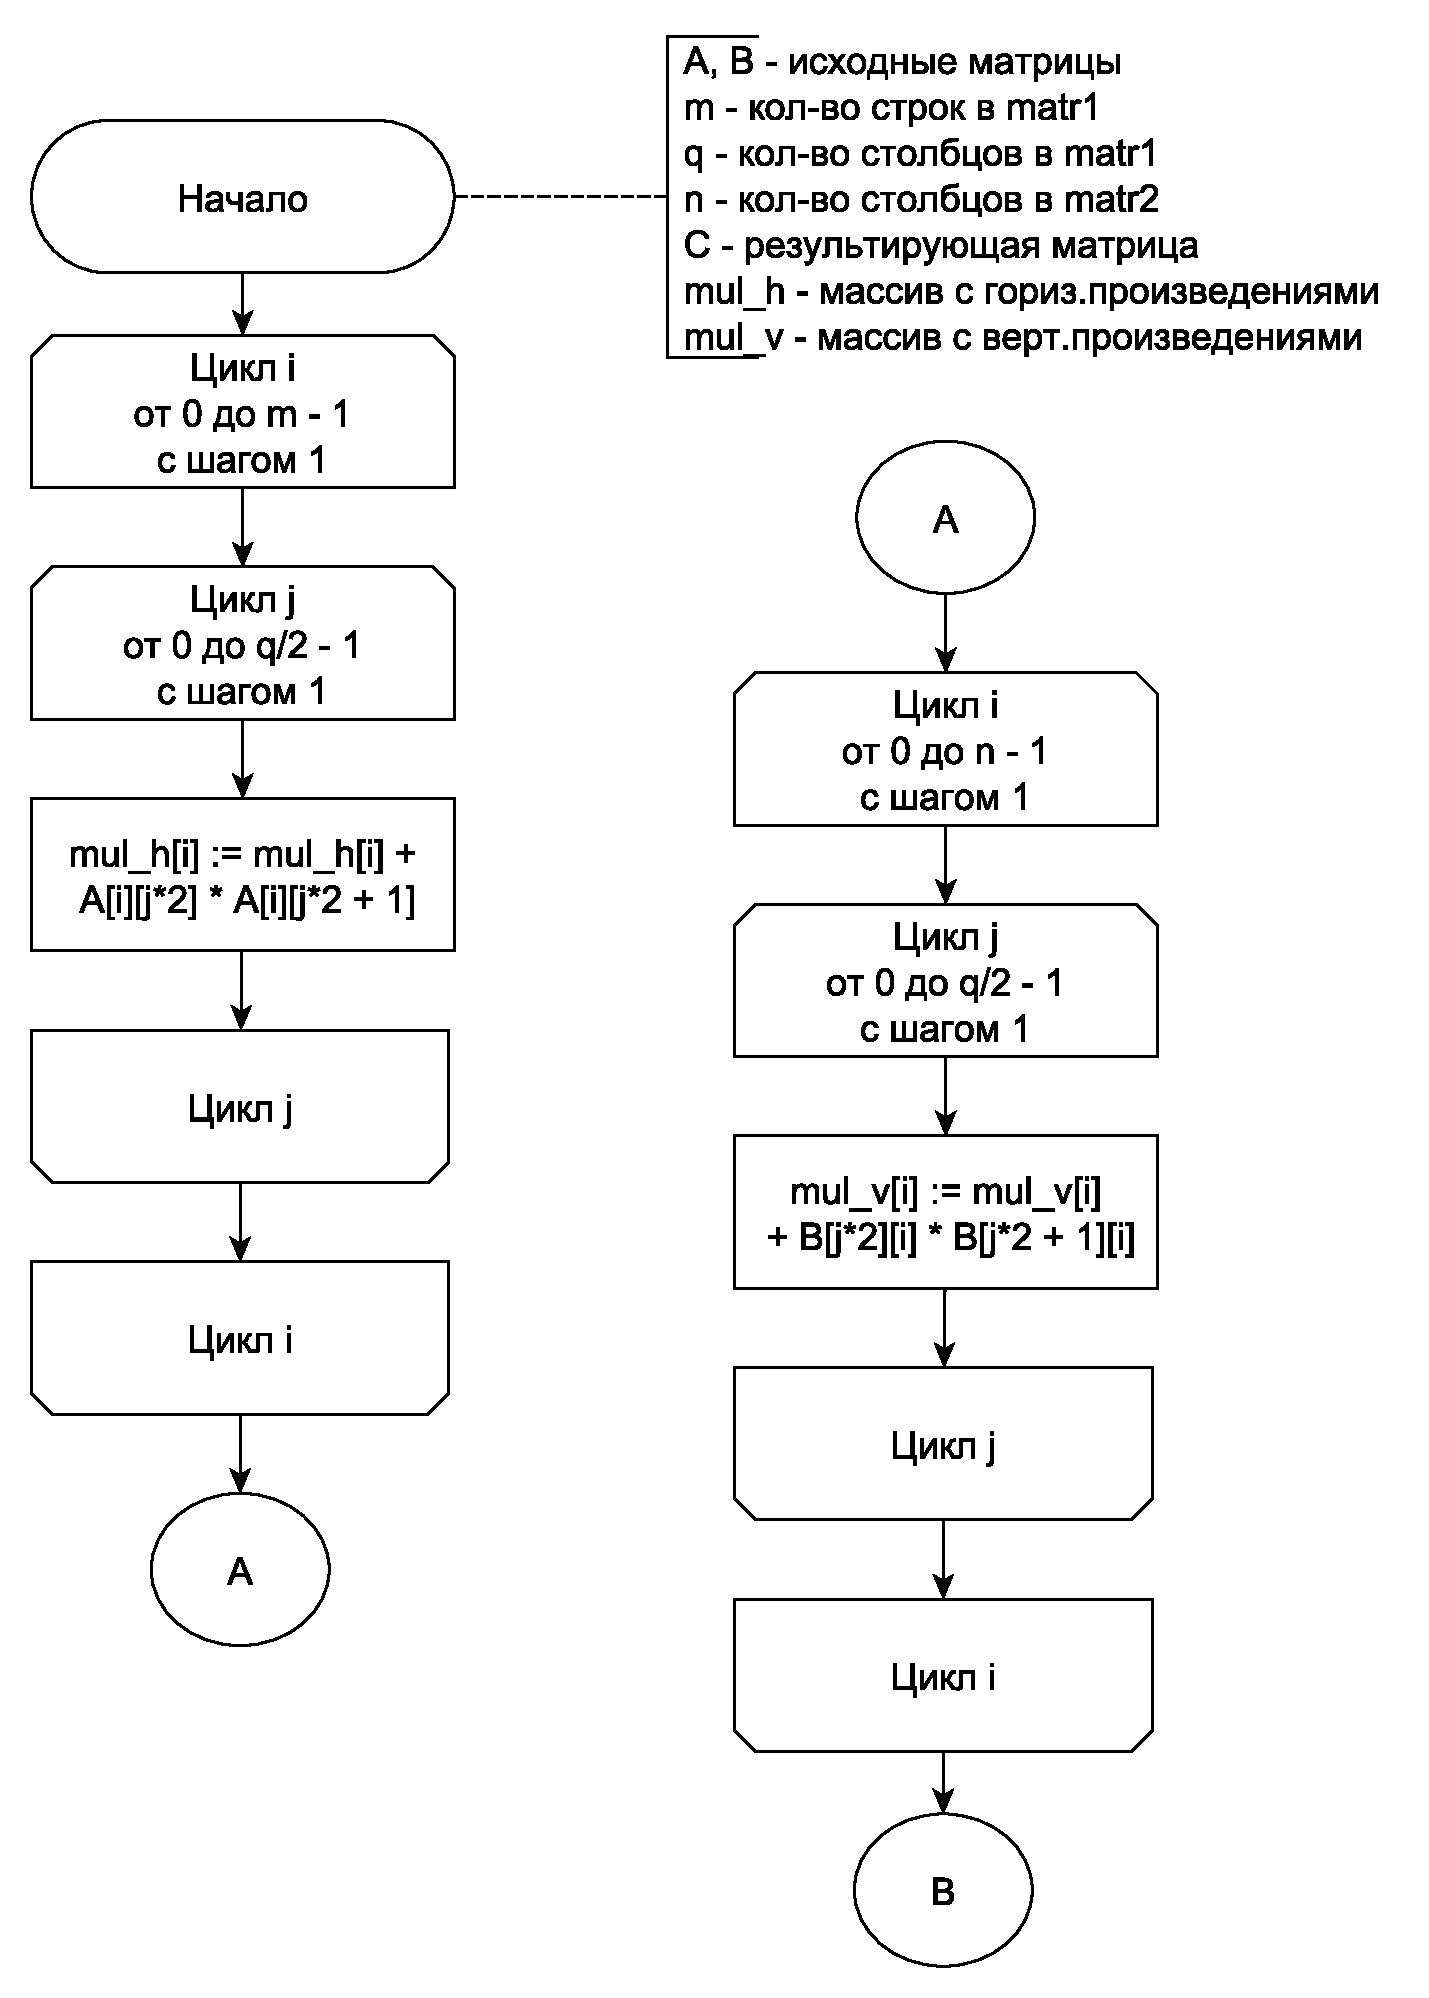
\includegraphics[scale = 0.5]{schema06.pdf}}
        		\caption{Схема алгоритма умножения матриц по Винограду (часть 1)}
        		\label{fig:schema_mult_v_1}
        	\end{center}
        \end{figure}
        
        \begin{figure}[h!]
        	\begin{center}
        		{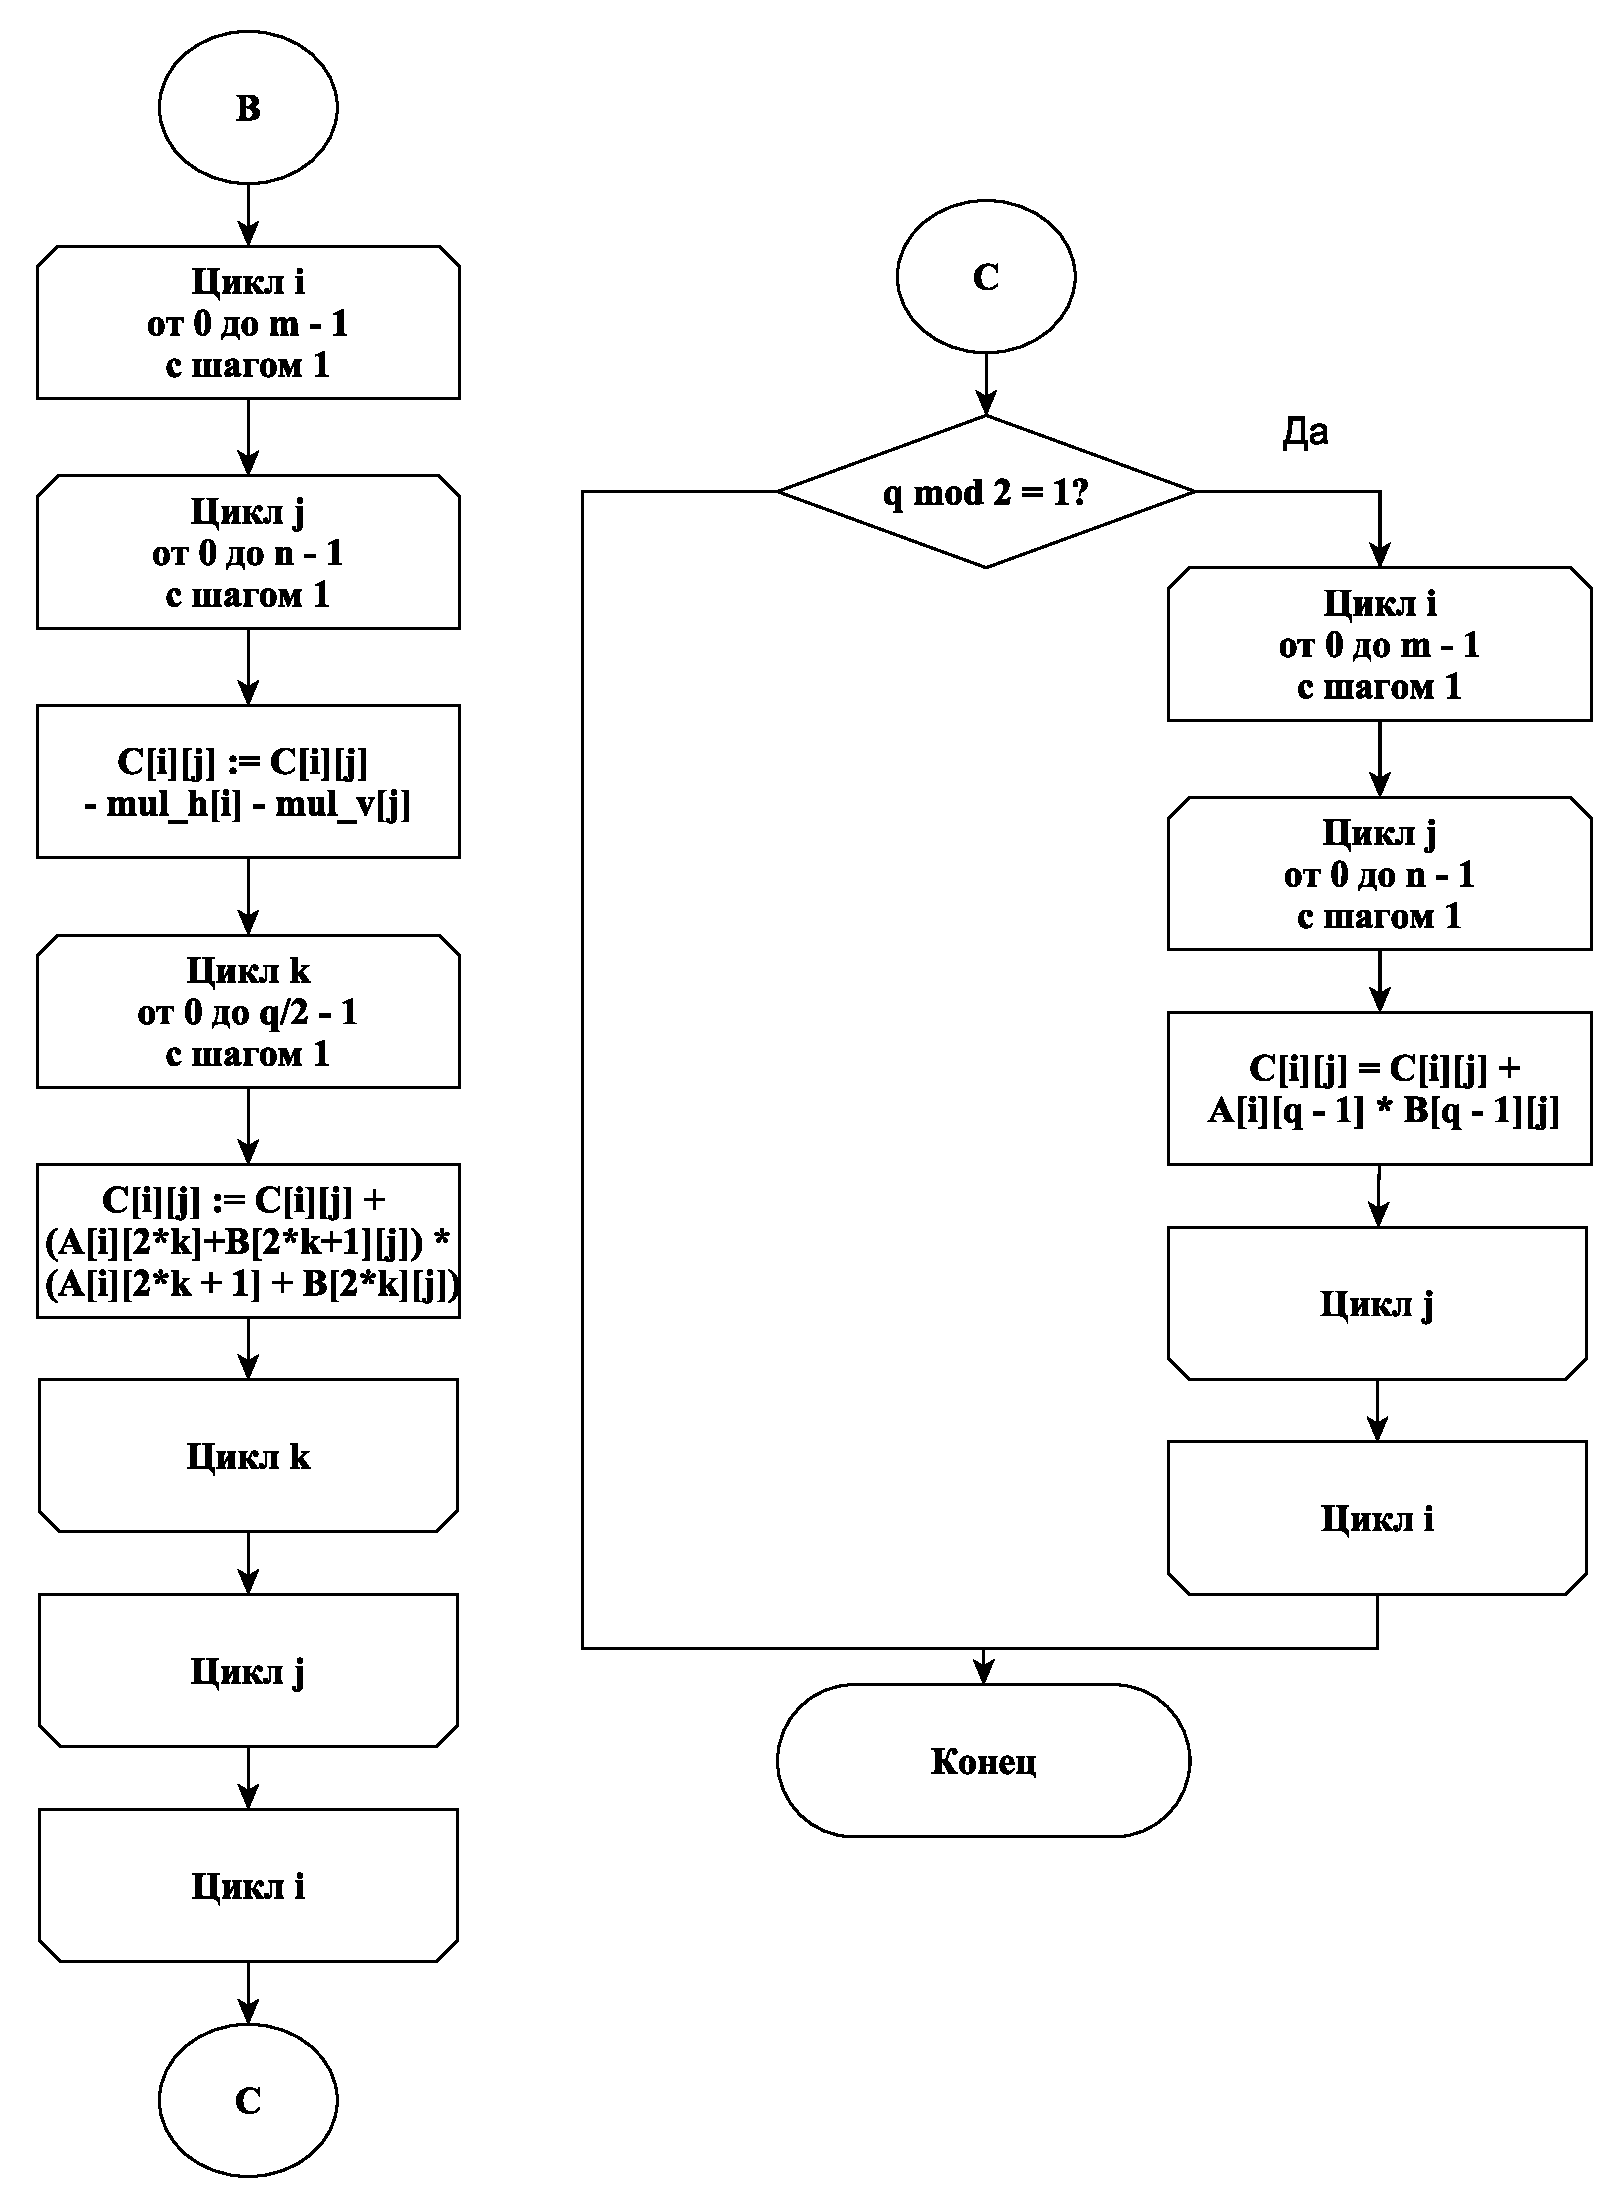
\includegraphics[scale = 0.5]{schema07.pdf}}
        		\caption{Схема алгоритма умножения матриц по Винограду (часть 2)}
        		\label{fig:schema_mult_v_2}
        	\end{center}
        \end{figure}
        
        \subsubsection{Оптимизация алгоритма Винограда}
        		Заполнение массива под горизонтальные (вертикальные) произведения:
	\begin{enumerate} 
	\item[1)] замена = на +=;
	\item[2)] замена во внутреннем цикле шага цикла с 1 на 2 $\Rightarrow$ происходит замена j*2 на j.
	\end{enumerate}
	
	Тройной цикл:
	\begin{enumerate} 
	\item[1)] замена = на +=;
	\item[2)] замена в цикле по q шага цикла с 1 на 2 $\Rightarrow$ происходит замена k*2 на k;
	\item[3)] вычисление $q2 = q - 1$ заранее;
	\item[4)] использование буфера для накопления результата по циклу q и занесение результата в $res\_matr[i][j]$ после цикла;
	\item[5)] вычисление горизонтального и вертикального произведения заранее отрицательным.

	\end{enumerate}
	
	Условный переход:
	\begin{enumerate} 
	\item[1)] замена = на +=;
	\item[2)] замена во внутреннем цикле шага цикла с 1 на 2 $\Rightarrow$ происходит замена j*2 на j;
	\item[3)] вычисление q2 = q - 1 заранее.
	\end{enumerate}
    
    \subsubsection{Реализация многопоточности}
    Пусть разрешено использовать до N рабочих потоков, тогда распараллелить алгоритм Винограда можно следующими способами.
	  \begin{enumerate}
	  \item[1)] Выполнять вычисления горизонтальных и вертикальных произведений в двух рабочих потоках.
	  \item[2)] В тройном цикле организовать внешний цикл так, чтобы первый рабочий поток вычислял элементы первой строки результирующей матрицы, затем элементы (1 + N)-ой строки, элементы (1 + 2*N)-ой строки и т.д., второй рабочий поток аналогично вычисляет строки 2, 2 + N, 2 + 2*N, ... . Таким образом i-й рабочий поток вычисляет строки i, i + N, i + 2*N, ... , пока i < m, где m - длина первой матрицы.
	  \item[3)] Аналогично 2) организовать внешний цикл в условном переходе.
	  \end{enumerate}
	  
	  Таким образом, сначала происходит параллельный расчёт горизонтальных и вертикальных произведений в двух рабочих потоках, затем каждая строка результирующей матрицы вычисляется на отдельном рабочем потоке и затем, если матрица нечетной размерности, дополнительные вычисления (в условном переходе) аналогично выполняются для каждой строки результирующей матрицы на отдельном рабочем потоке.
	    
	На рис. \ref{fig:schema_main}, \ref{fig:schema_h}, \ref{fig:schema_v}, \ref{fig:schema_m} и \ref{fig:schema_in_if} представлены схемы оптимизированного алгоритма Винограда, разбитого на потоки.
	    \begin{figure}[h!]
	    	\begin{center}
	    		{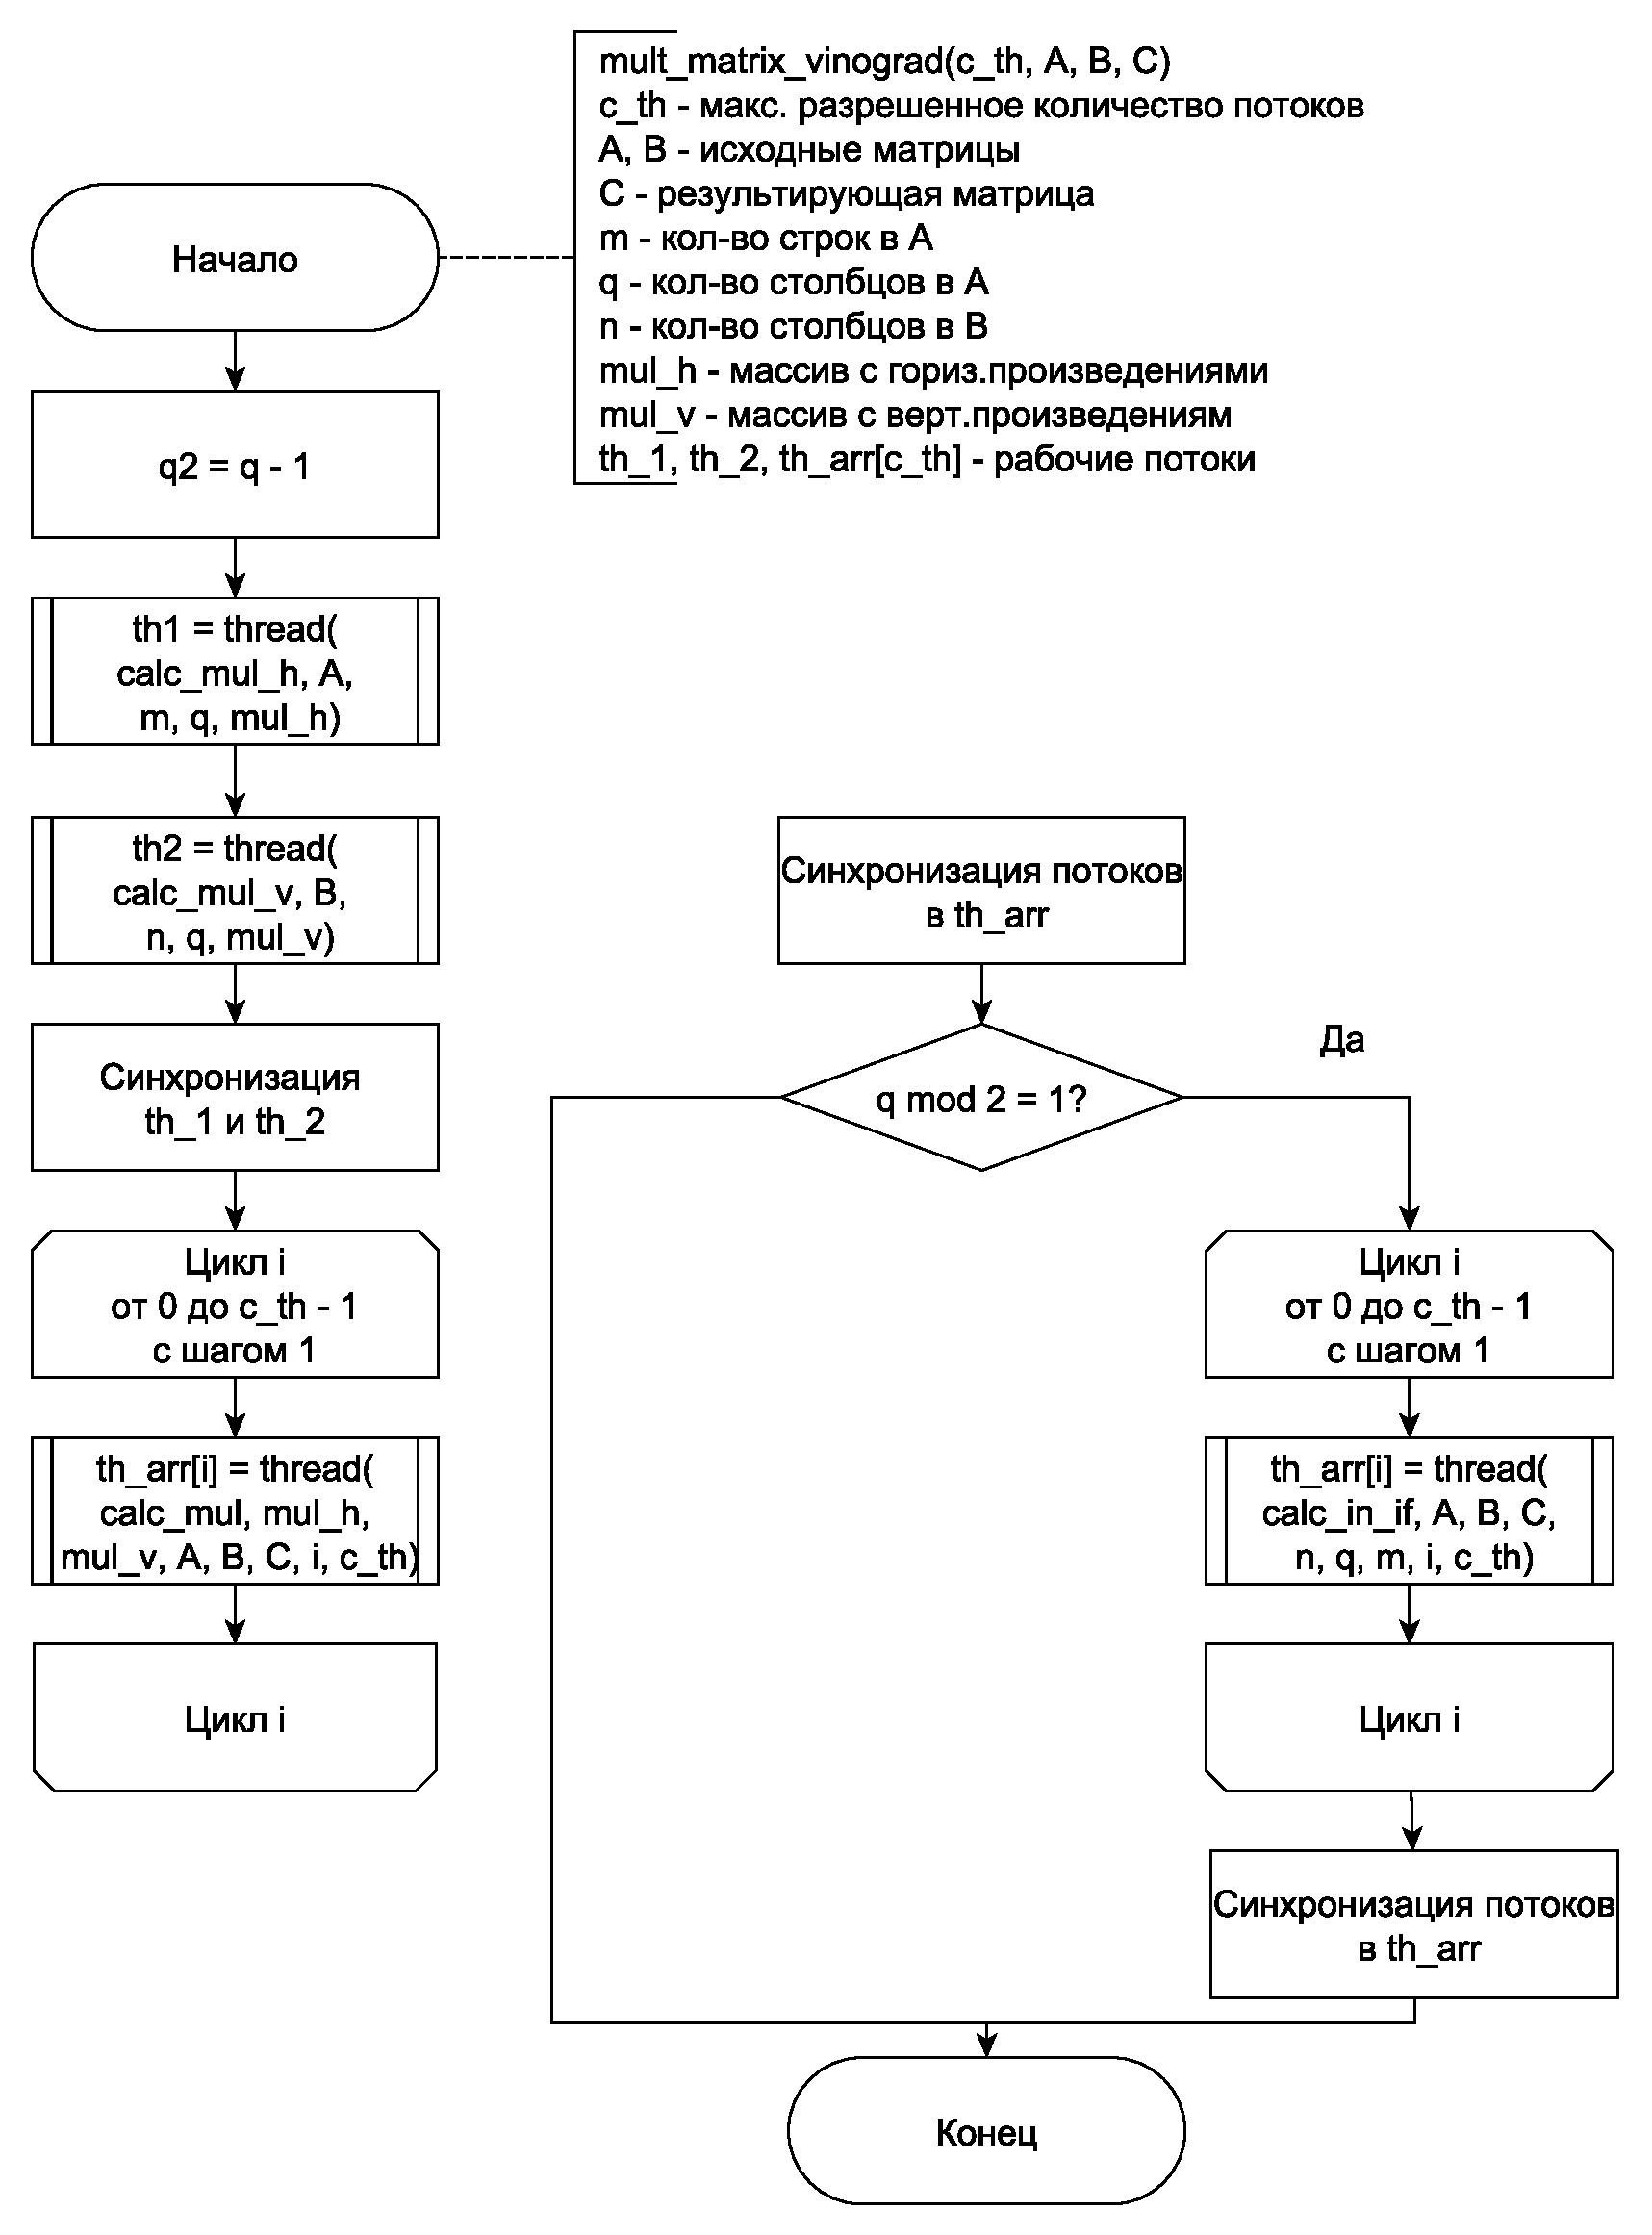
\includegraphics[scale = 0.5]{schema01.pdf}}
	    		\caption{Схема основной функции}
	    		\label{fig:schema_main}
	    	\end{center}
	    \end{figure}
	    
	    	    \begin{figure}[h!]
	    	\begin{center}
	    		{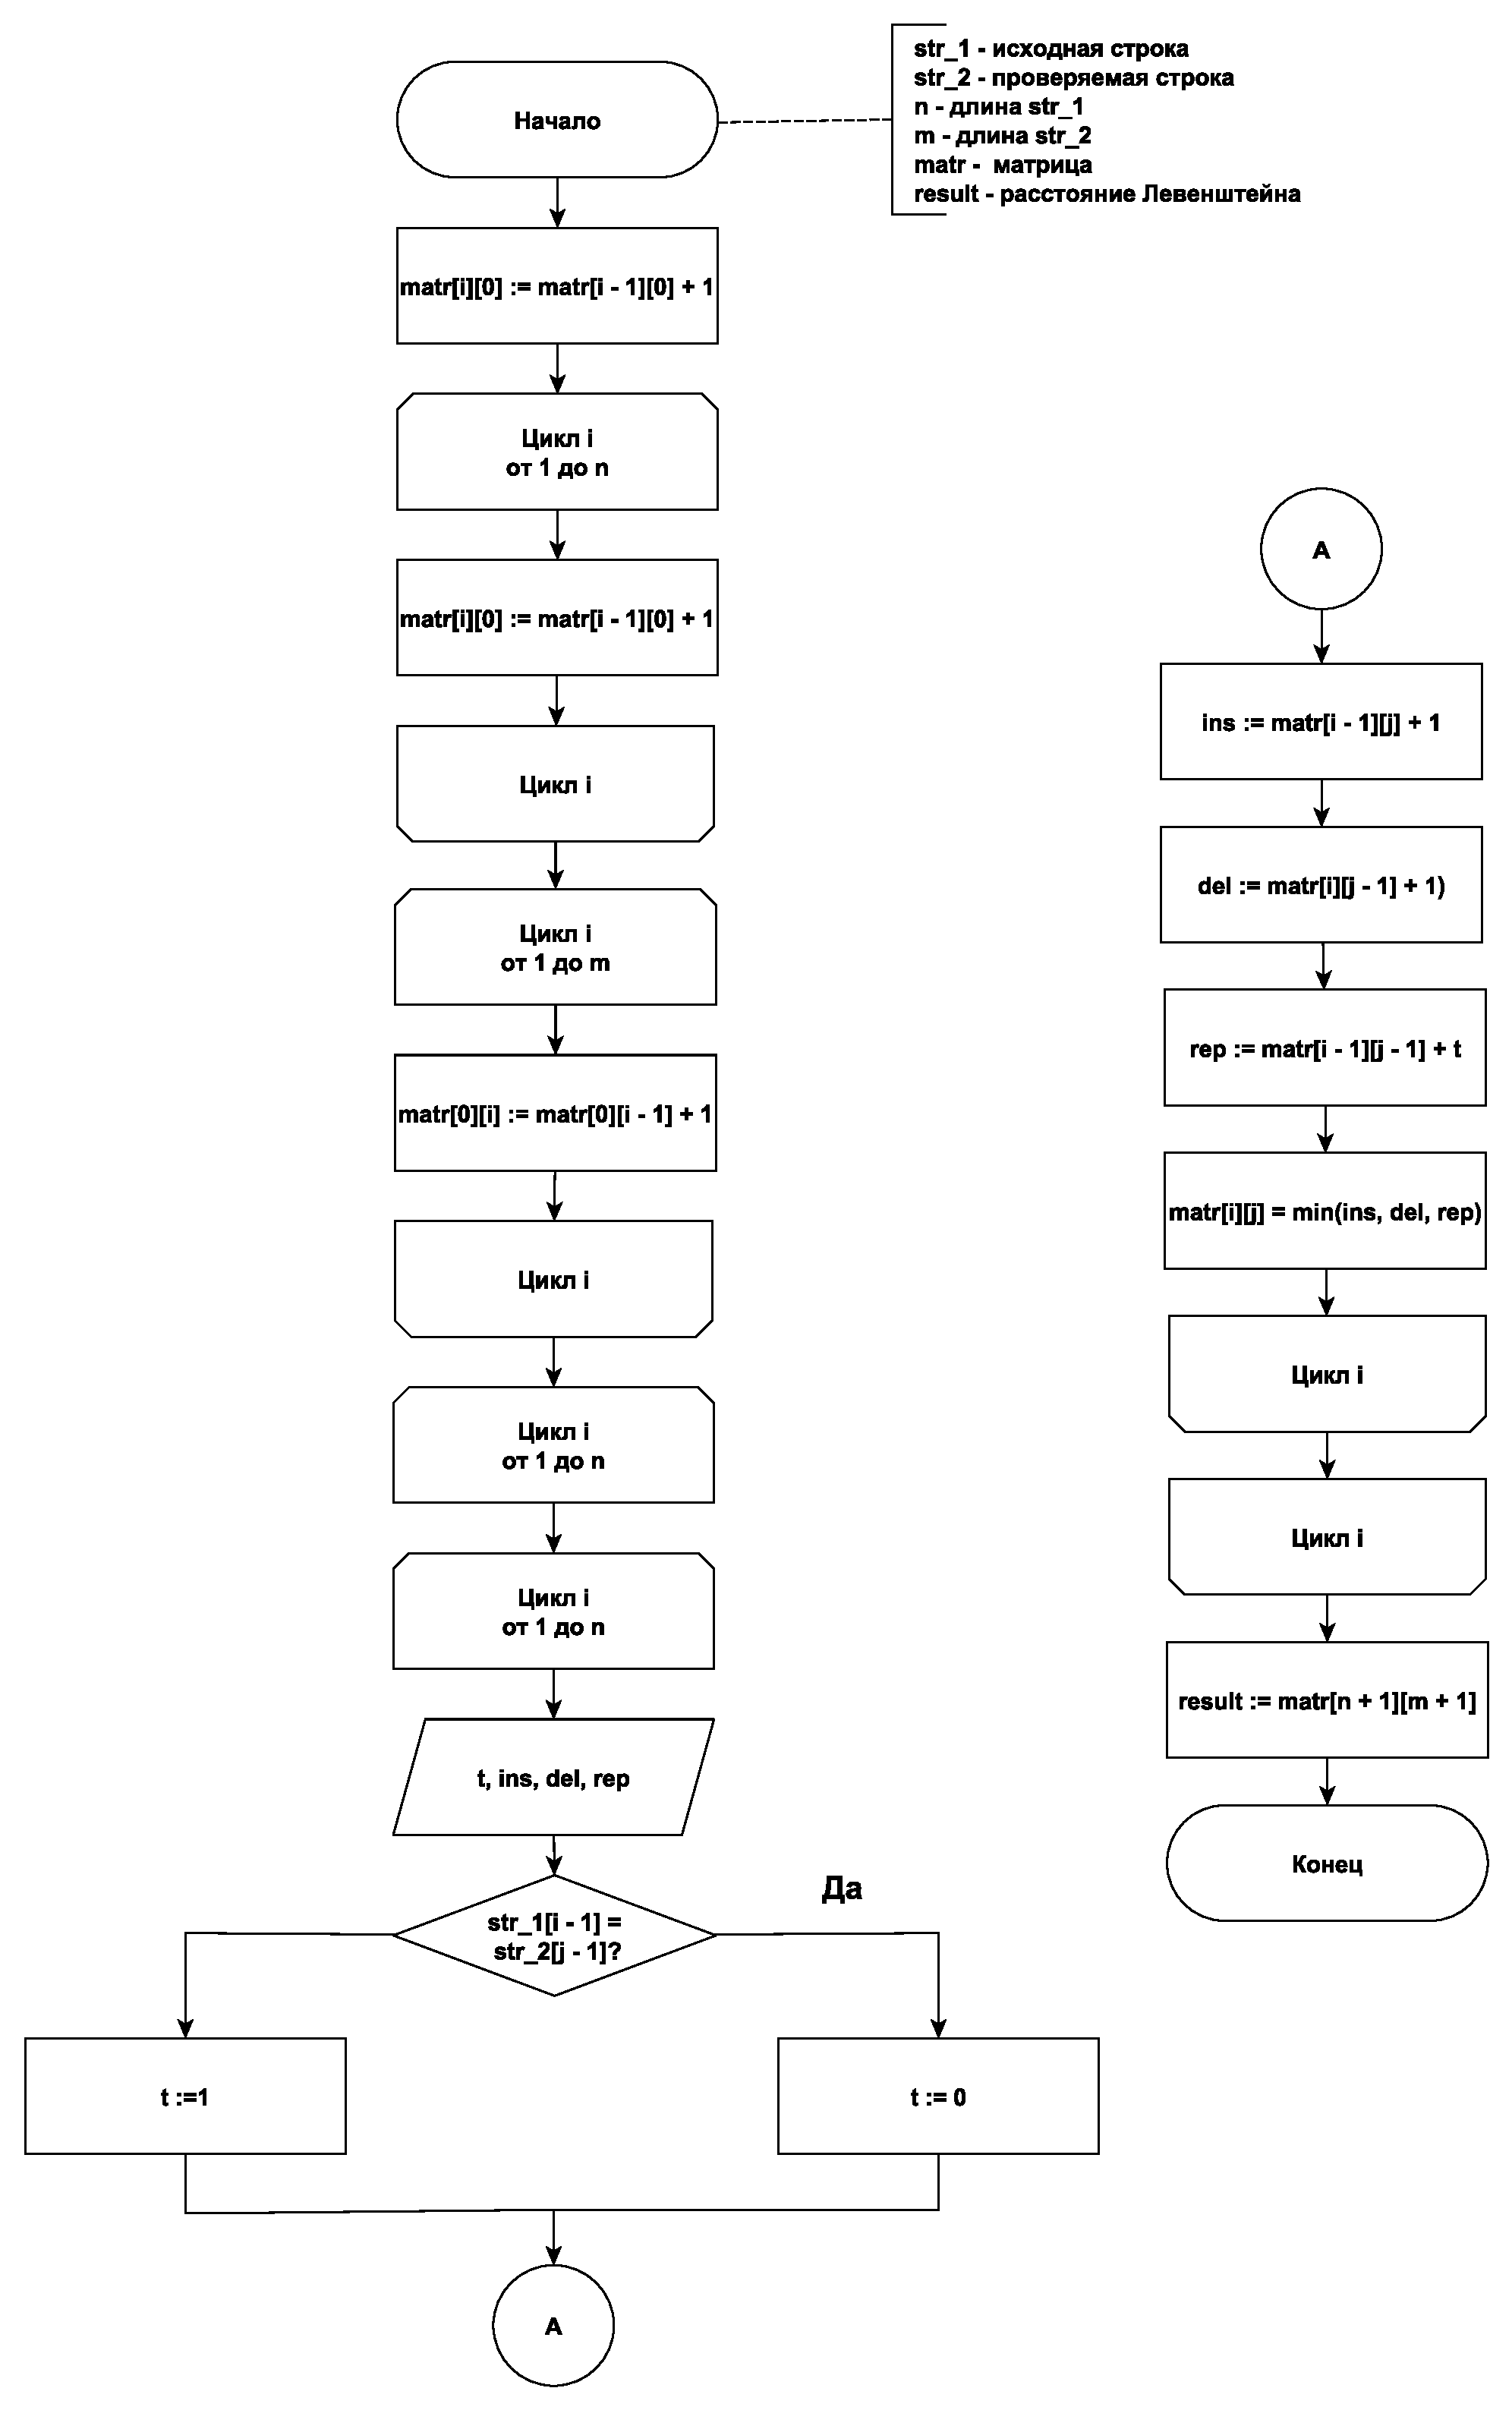
\includegraphics[scale = 0.5]{schema02.pdf}}
	    		\caption{Схема функции, вычисляющей горизонтальные произведений}
	    		\label{fig:schema_h}
	    	\end{center}
	    \end{figure}
	    
	    	    \begin{figure}[h!]
	    	\begin{center}
	    		{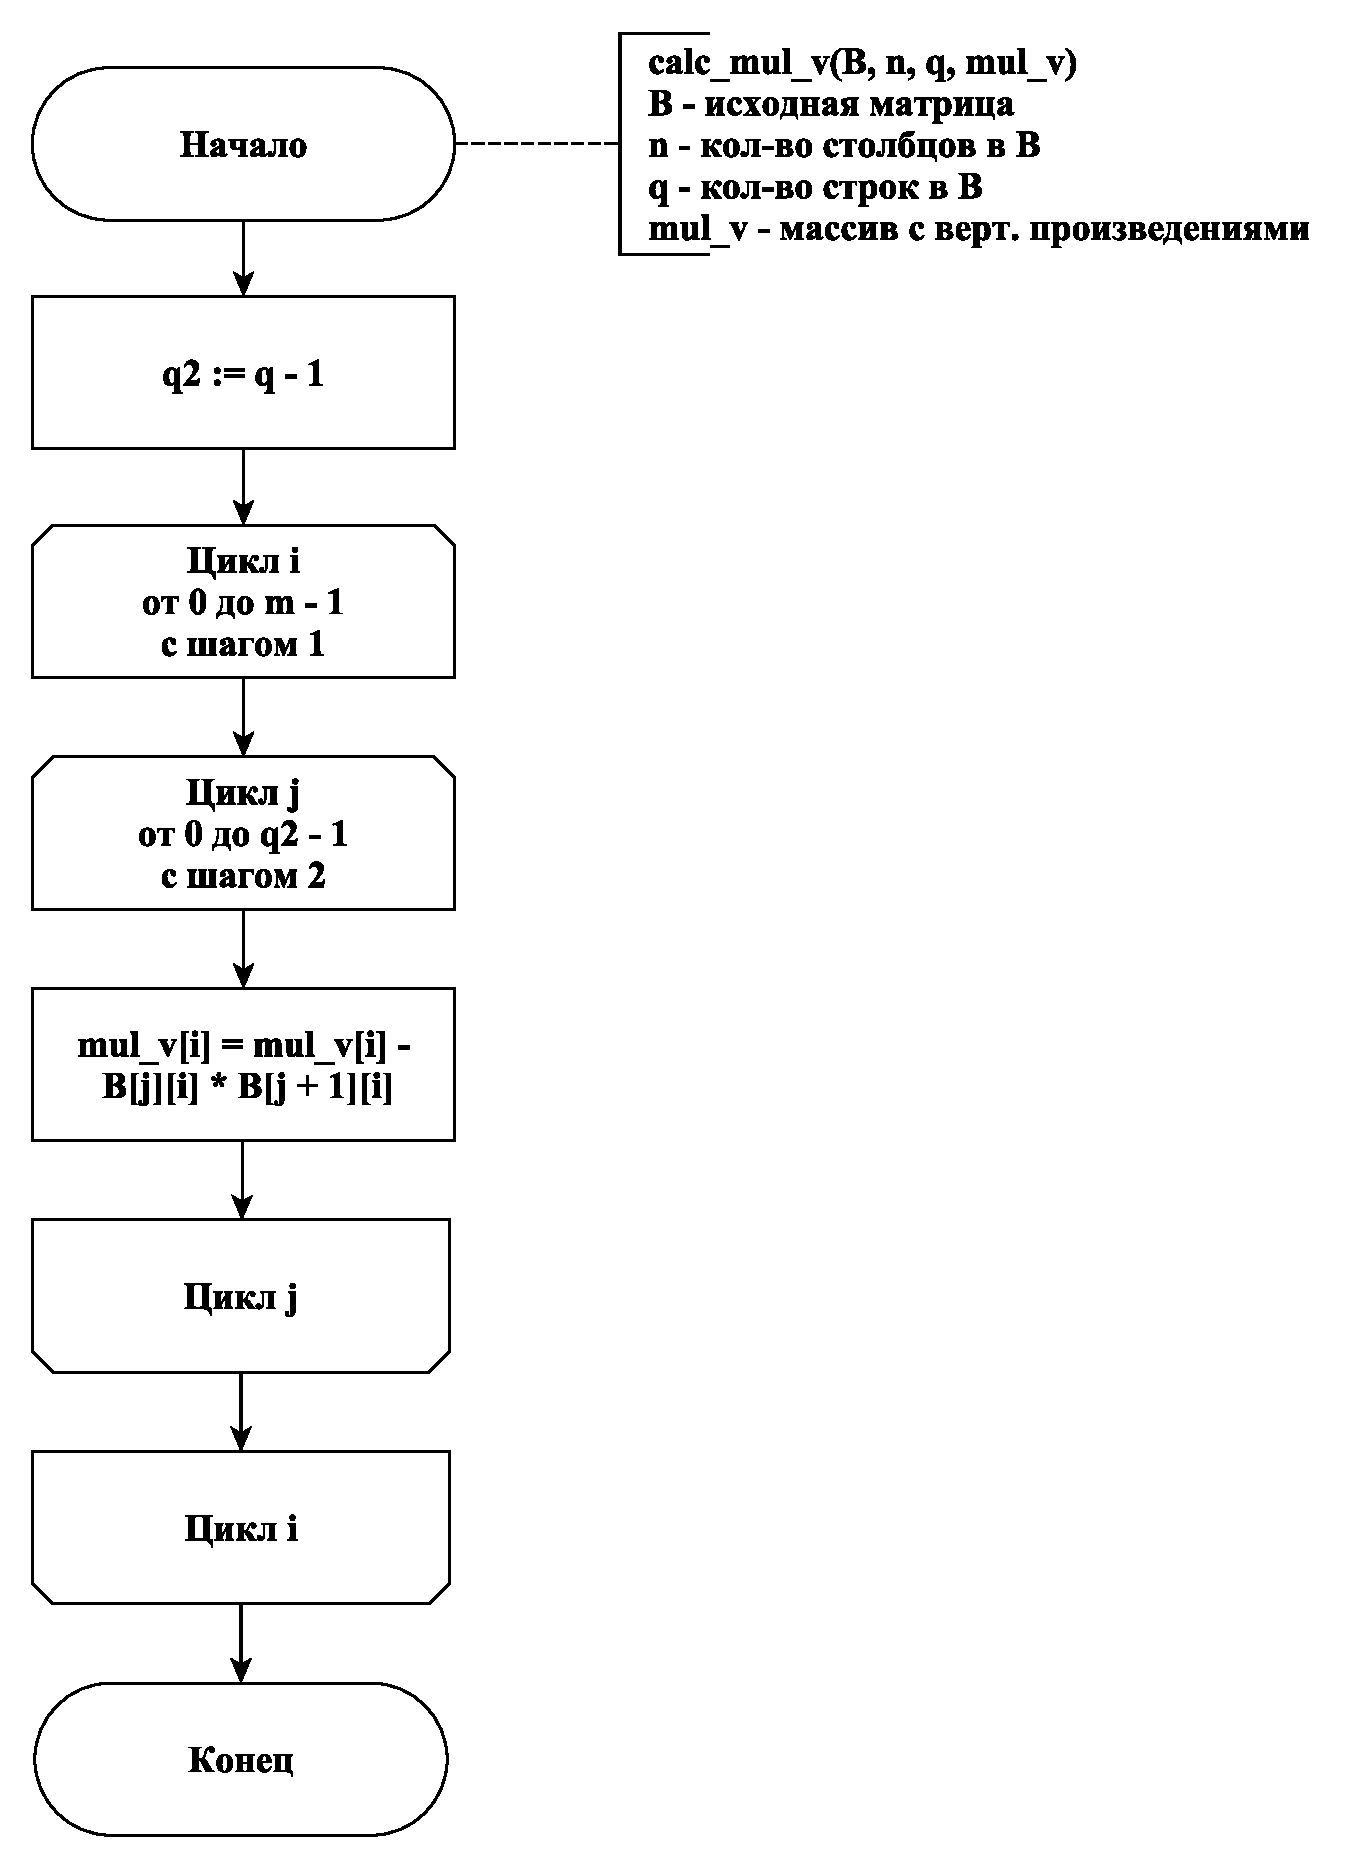
\includegraphics[scale = 0.5]{schema03.pdf}}
	    		\caption{Схема функции, вычисляющей горизонтальные произведений}
	    		\label{fig:schema_v}
	    	\end{center}
	    \end{figure}
	    
	    	    \begin{figure}[h!]
	    	\begin{center}
	    		{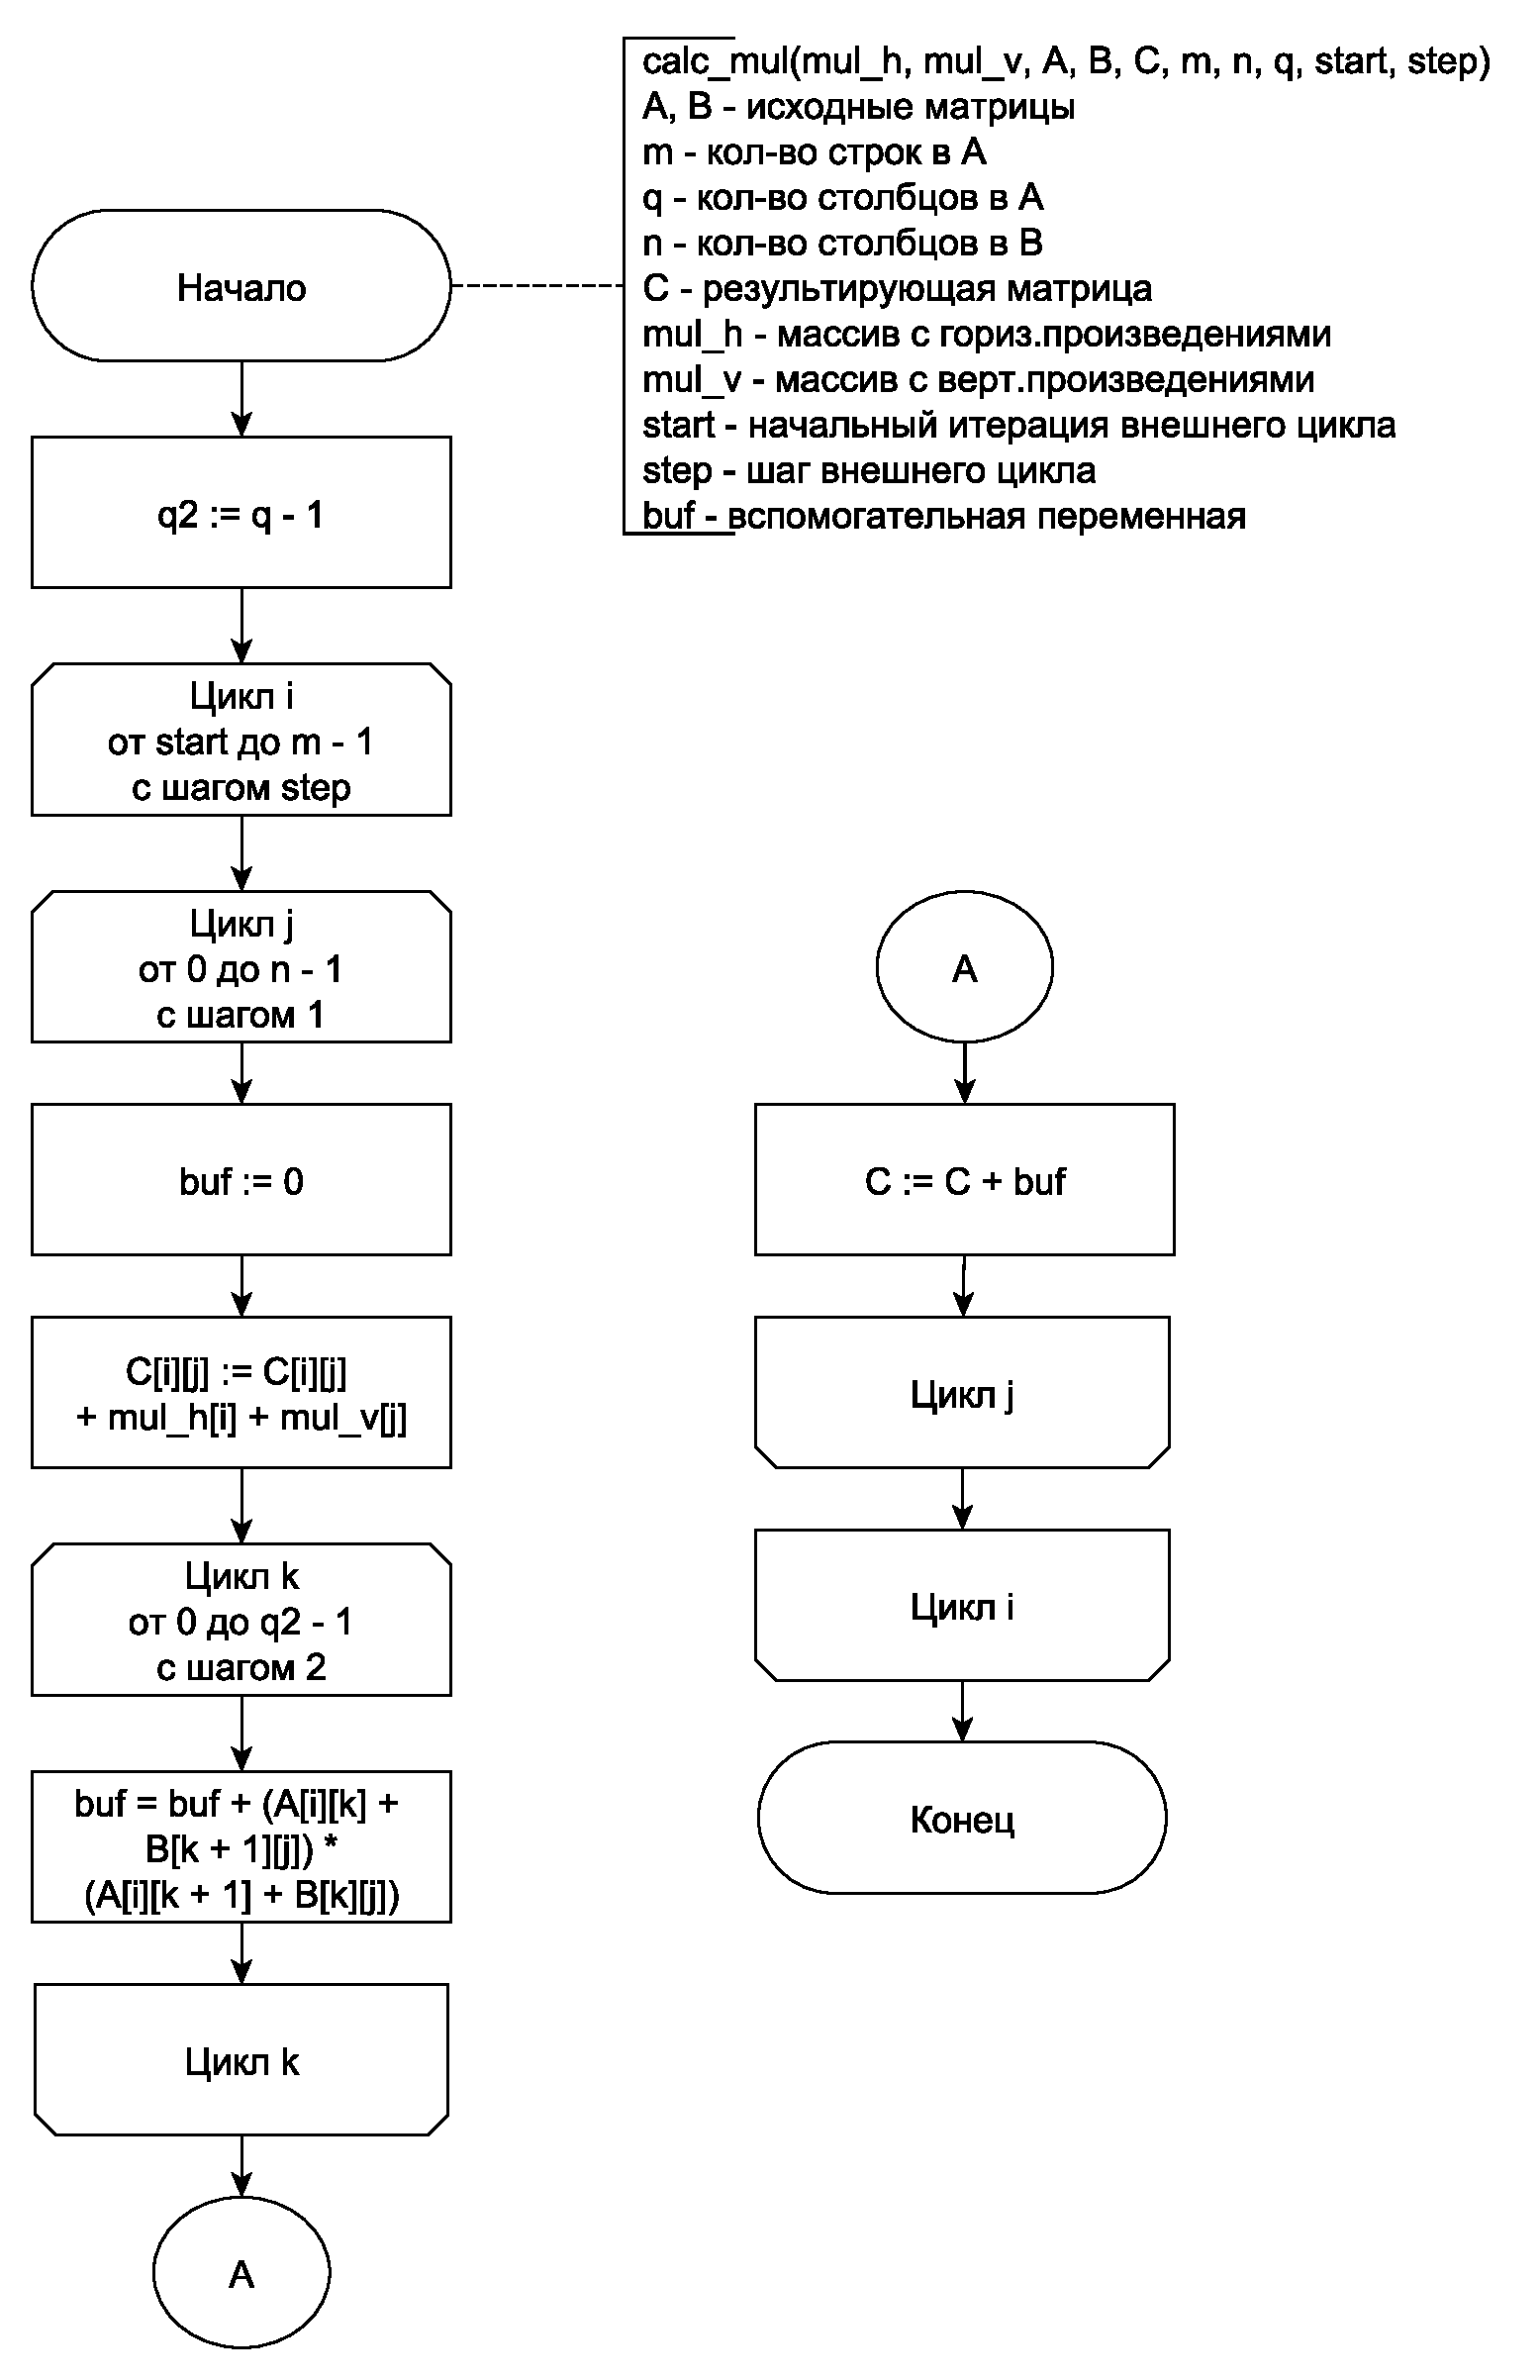
\includegraphics[scale = 0.5]{schema04.pdf}}
	    		\caption{Схема функции вычислений в тройном цикле}
	    		\label{fig:schema_m}
	    	\end{center}
	    \end{figure}
	    
	    
	    	    \begin{figure}[h!]
	    	\begin{center}
	    		{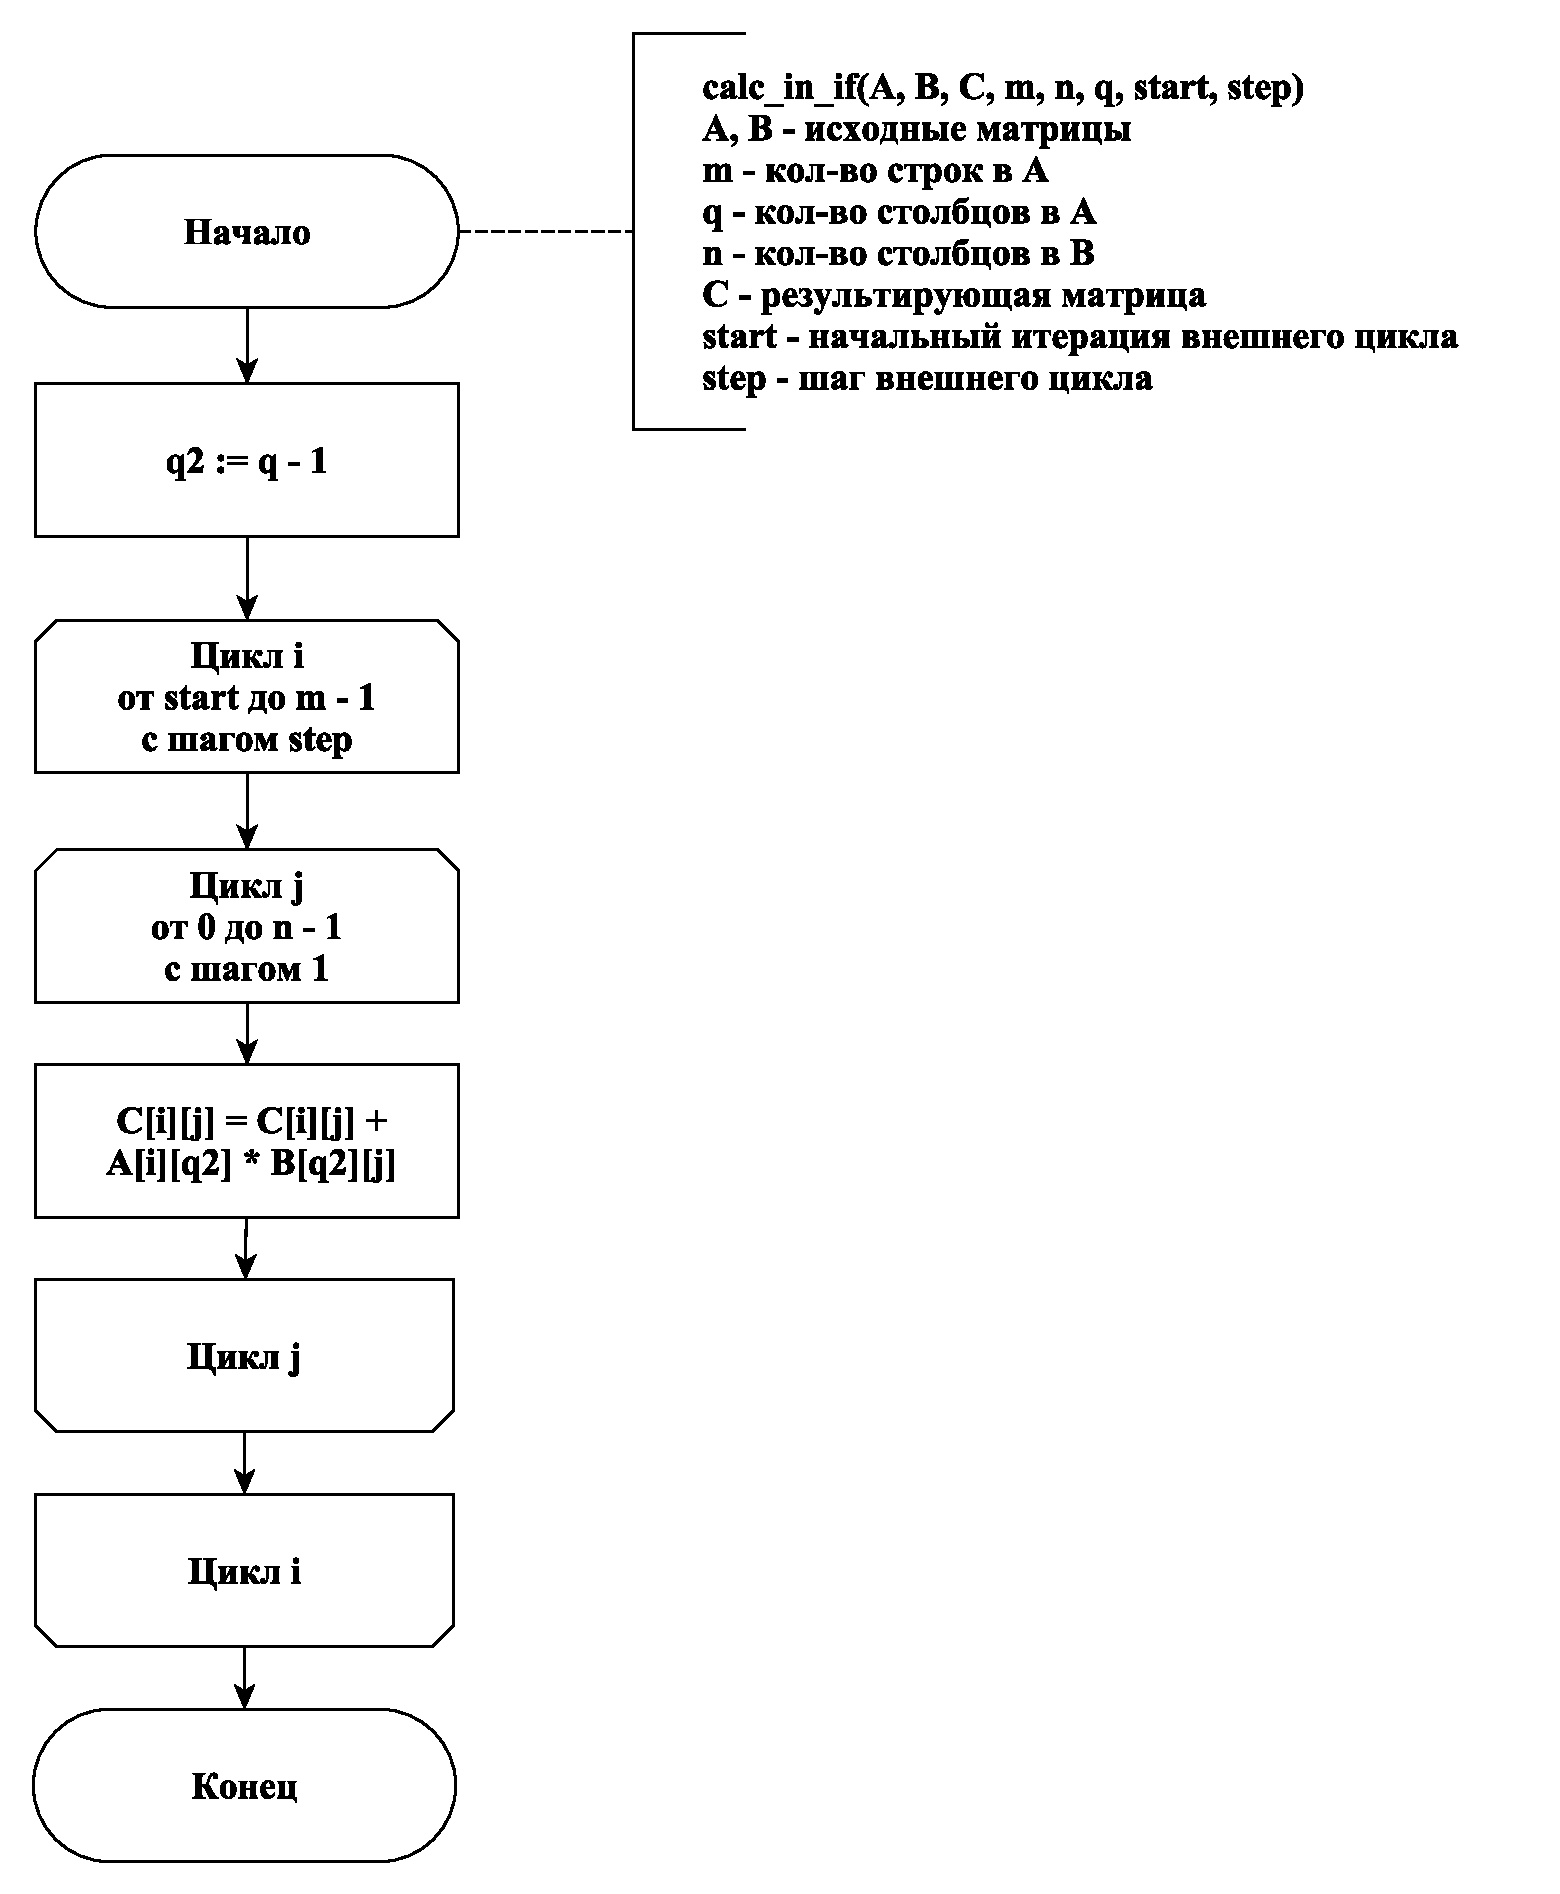
\includegraphics[scale = 0.5]{schema05.pdf}}
	    		\caption{Схема функции вычислений внутри условного перехода}
	    		\label{fig:schema_in_if}
	    	\end{center}
	    \end{figure}
	    
	\newpage
	\mbox{}
	\newpage
	\mbox{}
	\newpage
	\mbox{}
	\newpage
	\mbox{}
	\newpage
	    
	    
	\subsection*{Вывод}
		\addcontentsline{toc}{subsection}{Вывод}
		В данном разделе были описаны шаги по оптимизации алгоритма Винограда, была предложена модификация алгоритма для многопоточного выполнения и были представлены схемы оптимизированного алгоритма Винограда и оптимизированного алгоритма Винограда, адаптированного под выполнение на потоках.



  
\pagebreak
\newpage         

\section{Технологический раздел}

	В данном разделе будут описаны требования к программному обеспечению и средства реализации, приведены листинг программ и тестовые данные.
	\subsection{Требования к программному обеспечению}
	Входные данные: 
	 \begin{enumerate} 
	 \item[1)] три целых положительных числа - размерности матриц: M, N и Q.
	 \item[2)] две матрицы размера M x Q и Q x N, заполненные целыми числами
	 \item[3)] целое число - максимальное количество рабочих потоков 
	 \end{enumerate}
	
	Выходные данные: матрица размера M x N, полученная в результате умножения исходных, с помощью оптимизированного алгоритма Винограда, разбитого на потоки.
	
	На рис. \ref{fig:idef0} приведена функциональная схема вычисления произведения матриц по оптимизированному алгоритму Винограда с разбиением на потоки.
        
        \begin{figure}[h!]
        	\begin{center}
        		{\includegraphics[width = \textwidth]{idef0.png}}
        		\caption{Функциональная схема вычисления произведения матриц по оптимизированному алгоритму Винограда с разбиением на потоки}
        		\label{fig:idef0}
        	\end{center}
        \end{figure}
        
	
	\subsection{Средства реализации}
	Программа написана на языке С++, т. к. этот язык предоставляет программисту широкие возможности реализации самых разнообразных алгоритмов, обладает высокой эффективностью и значительным набором стандартных классов и процедур. В качестве среды разработки использовалась среда разработки CLion.
	
	Для обработки матриц был использован стандартный контейнерный класс std::vector.
	
	Для замера времени выполнения программы использовалась библиотека chrono.
	

    
    \subsection{Листинг программы}
	В листинге \ref{code_main} содержится основная функция умножения матриц по оптимизировнаному алгоритму Винограду с разделением на потоки. В листингах \ref{code_h},  \ref{code_v}, \ref{code_m} и \ref{code_if} представлены функции, которые обрабатываются на рабочих потоках. 

		\begin{lstlisting}[label=code_main, caption={Основная функция}]
	void mult_matrix_vinograd_optimiz(int count_th, Matrix matr_1, Matrix matr_2,
                                  Matrix &res_matr) {
    size_t m = matr_1.size();
    size_t q = matr_1[0].size();
    size_t q2 = q - 1;
    size_t n = matr_2[0].size();

    Vector mul_h(m, 0);
    Vector mul_v(n, 0);

    std::thread thread_1(calc_mul_h, std::ref(matr_1), m, q2,
    										std::ref(mul_h));
    std::thread thread_2(calc_mul_v, std::ref(matr_2), n, q2,
    										std::ref(mul_v));
    thread_1.join();
    thread_2.join();

    std::vector<std::thread> thread_arr(count_th);

    for(int i = 0; i < count_th; i++) {
        thread_arr[i] = std::thread(calc_mult, std::ref(mul_h),
                                    std::ref(mul_v), std::ref(matr_1),
                                    std::ref(matr_2),
                                    std::ref(res_matr), i, count_th);
    }
    for(int i = 0; i < count_th; i++) {
        thread_arr[i].join();
    }

    if (q % 2 == 1) {
        for(int i = 0; i < count_th; i++) {
            thread_arr[i] = std::thread(calc_in_if, std::ref(matr_1), std::ref(matr_2), std::ref(res_matr), i, count_th);
        }
        for(int i = 0; i < count_th; i++) {
            thread_arr[i].join();
        }
    }
}
	\end{lstlisting}  
	
	\begin{center}
	\begin{lstlisting}[label=code_h, caption={Функция вычисления горизонтальных произведений}]
using Matrix = std::vector<std::vector<int>>;
using Vector = std::vector<int>;

void calc_mul_h(Matrix &matr_1, size_t m, size_t q2, Vector &mul_h) {
    for(size_t i = 0; i < m; i++) {
        for (size_t j = 0; j < q2; j+=2) {
            mul_h[i] -= matr_1[i][j] * matr_1[i][j + 1];
        }
    }
}


    \end{lstlisting}
    \end{center}  

     
	\begin{lstlisting}[label=code_v, caption={Функция вычисления вертикальных произведений}]
void calc_mul_v(Matrix &matr_2, size_t n, size_t q2, Vector &mul_v) {
    for(size_t i = 0; i < n; i++) {
        for (size_t j = 0; j < q2; j+=2) {
            mul_v[i] -= matr_2[j][i] * matr_2[j + 1][i];
        }
    }
}

\end{lstlisting}


	\begin{lstlisting}[label=code_m, caption={Функция вычислений в тройном цикле}]
void calc_mult(Vector &mul_h, Vector &mul_v, Matrix &matr_1, Matrix &matr_2,
               Matrix &res_matr, size_t start, size_t step) {
    size_t m = matr_1.size();
    size_t q2 = matr_1[0].size() - 1;
    size_t n = matr_2[0].size();
    for(size_t i = start; i < m; i += step) {
        for (size_t j = 0; j < n; j++) {
            res_matr[i][j] = mul_h[i] + mul_v[j];
            int buf = 0;
            for(size_t k = 0; k < q2; k+=2) {
                buf += (matr_1[i][k] + matr_2[k + 1][j]) *
                                    (matr_1[i][k + 1] + matr_2[k][j]);
            }
            res_matr[i][j] += buf;
        }
    }
}

    \end{lstlisting}  
    
    
	\begin{lstlisting}[label=code_if, caption={Функция дополнительных вычислений для матриц нечетной размерности }]
	void calc_in_if(Matrix &matr_1, Matrix &matr_2, Matrix &res_matr, 											size_t start, size_t step) {
    size_t m = matr_1.size();
    size_t q2 = matr_1[0].size() - 1;
    size_t n = matr_2[0].size();
    for(size_t i = start; i < m; i += step) {
        for (size_t j = 0; j < n; j++) {
            res_matr[i][j] += matr_1[i][q2] * matr_2[q2][j];
        }
    }
}
	\end{lstlisting}  
	

    
%    
    \subsection{Тестовые данные}
    \label{fig:test_data}

    Программа должна корректно умножать матрицы при следующих входных данных при количестве рабочих потоков от 1 до 128 (1, 2, 4, 8, 16, ... , 128):
\\
\begin{enumerate}
	\item[1)] матрицы $1 \times 1$:
	\[ \begin{bmatrix}
2
\end{bmatrix} \times 
\begin{bmatrix}
3
\end{bmatrix} =
\begin{bmatrix}
6
\end{bmatrix}; \]

	\item[2)] умножение на нулевую матрицу:
	\[ \begin{bmatrix}
1 & 2 \\
3 & 4
\end{bmatrix} \times 
\begin{bmatrix}
0 & 0 \\
0 & 0
\end{bmatrix} =
\begin{bmatrix}
0 & 0 \\
0 & 0
\end{bmatrix}; \]

	\item[3)] умножение на единичную матрицу:
\[ \begin{bmatrix}
1 & 2 \\
3 & 4
\end{bmatrix} \times 
\begin{bmatrix}
1 & 0 \\
0 & 1
\end{bmatrix} =
\begin{bmatrix}
1 & 2 \\
3 & 4
\end{bmatrix}; \]

		\item[4)] умножение(матрицы $2 \times 2$) на матрицу с положительными числами:
\[ \begin{bmatrix}
1 & 2 \\
3 & 4
\end{bmatrix} \times 
\begin{bmatrix}
1 & 2 \\
3 & 4
\end{bmatrix} =
\begin{bmatrix}
7 & 10 \\
15 & 22
\end{bmatrix}; \]

		\item[5)] умножение (матрицы $2 \times 2$) на матрицу отрицательными числами:
\[ \begin{bmatrix}
1 & 2 \\
3 & 4
\end{bmatrix} \times 
\begin{bmatrix}
-1 & -2 \\
-3 & -4
\end{bmatrix} =
\begin{bmatrix}
-7 & -10 \\
-15 & -22
\end{bmatrix}; \]


		\item[6)] умножение (матрицы $3 \times 3$) на матрицу с положительными числами:
\[ \begin{bmatrix}
1 & 2 & 3 \\
4 & 5 & 6 \\
7 & 8 & 9 
\end{bmatrix} \times 
\begin{bmatrix}
1 & 2 & 3 \\
4 & 5 & 6 \\
7 & 8 & 9 
\end{bmatrix} =
\begin{bmatrix}
30 & 36 & 42 \\
66 & 81 & 96 \\
102 & 126 & 150 
\end{bmatrix}; \]

		\item[7)] умножение (матрицы $3 \times 3$) на матрицу с отрицательными числами:
\[ \begin{bmatrix}
1 & 2 & 3 \\
4 & 5 & 6 \\
7 & 8 & 9 
\end{bmatrix} \times 
\begin{bmatrix}
-1 & -2 & -3 \\
-4 & -5 & -6 \\
-7 & -8 & -9 
\end{bmatrix} =
\begin{bmatrix}
-30 & -36 & -42 \\
-66 & -81 & -96 \\
-102 & -126 & -150 
\end{bmatrix}; \]

	\item[8)] умножение на прямоугольную матрицу с нечётным количеством столбцов:
\[ \begin{bmatrix}
1 & 2 & 3\\
4 & 5 & 6
\end{bmatrix} \times 
\begin{bmatrix}
1 & 2 \\
3 & 4 \\
5 & 6
\end{bmatrix} =
\begin{bmatrix}
22 & 28 \\
49 & 64
\end{bmatrix}; \]

	\item[9)] умножение на  прямоугольную матрицу с чётным количеством столбцов:
\[ \begin{bmatrix}
1 & 2 & 3 & 4\\
5 & 6 & 7 & 8
\end{bmatrix} \times 
\begin{bmatrix}
1 & 2 \\
3 & 4 \\
5 & 6 \\
7 & 8
\end{bmatrix} =
\begin{bmatrix}
50 & 60 \\
114 & 140
\end{bmatrix}; \]

	\item[10)] умножение матриц c большими числами:	
\[ \begin{bmatrix}
1000 & 2000 & 3000 \\
4000 & 5000 & 6000  \\
7000 & 8000 & 9000
\end{bmatrix} \times 
 \begin{bmatrix}
1000 & 2000 & 3000 \\
4000 & 5000 & 6000  \\
7000 & 8000 & 9000
\end{bmatrix} =
\begin{bmatrix}
30000000 & 36000000 & 42000000 \\
66000000 & 81000000 & 96000000 \\
102000000 & 126000000 & 150000000
\end{bmatrix}; \]

	\end{enumerate}
    	
    Все тесты успешно пройдены.
	

	
	
	\subsection*{Вывод}
		\addcontentsline{toc}{subsection}{Вывод}
	
	В данном разделе были рассмотрены требования к программному обеспечению, в качестве средств реализации выбраны язык С++ и среда разработки CLion, приведён листинг программы и тестовые данные. 

\pagebreak

\section{Исследовательский раздел}

    
    \subsection{Примеры работы}
        
        На рис. \ref{fig:image_test_1}, \ref{fig:image_test_2}, \ref{fig:image_test_3} и \ref{fig:image_test_4} приведены примеры работы программы для различных входных данных. 
        
        	\begin{figure}[h!]
                \center{\includegraphics[scale = 0.7]{test01.png}}
                \caption{Пример работы программы для некорректного ввода}
                \label{fig:image_test_1}
            \end{figure}
            
            
            \begin{figure}[h!]
                \center{\includegraphics[scale = 0.6]{test02.png}}
                \caption{Пример работы программы для матриц четной размерности ($2 \times 2$)}
                \label{fig:image_test_2}
            \end{figure}        
        
            \begin{figure}[h!]
                \center{\includegraphics[scale = 0.6]{test03.png}}
                \caption{Пример работы программы для матриц нечетной размерности ($2 \times 3$ и $3 \times 2$}
                \label{fig:image_test_3}
            \end{figure}
            
               \begin{figure}[h!]
                \center{\includegraphics[scale = 0.7]{test04.png}}
                \caption{Пример работы программы для большого количества рабочих потоков}
                \label{fig:image_test_4}
            \end{figure}
    \newpage
	\mbox{}
	\newpage


    \subsection{Постановка эксперимента}
    
    Необходимо выполнить следующие замеры времени:
    \begin{enumerate} 
        \item[1)] Сравнить время умножения матриц оптимизированным алгоритмом Винограда для последовательной реализации алгоритма и для параллельной реализации с одним рабочим потоком:
        \begin{enumerate}
        \item[1.1)] сравнение на матрицах размером от $100 \times 100$ до $1000 \times 1000$ с шагом 100
        \item[1.2)] сравнение на матрицах размером от $101 \times 101$ до $1001 \times 1001$ с шагом 100
        \end{enumerate}
        \item[2)] Сравнить время умножения матриц оптимизированным алгоритмом Винограда для параллельной реализации с количеством рабочих потоков от 1 до 32 (количество потоков меняется как геометрическая прогрессия с шагом 2).
    \end{enumerate}
    
    Каждый замер производится 10 раз, а затем находится среднее значение. 
    
    
    \subsection{Сравнительный анализ на материале экспериментальных данных}
    	Замеры были произведены на 4-ядерном процессоре Intel Core i7 с тактовой частотой 3,5 ГГц с 8-ю логическими потоками, оперативная память — 16 ГБ.
    	
    	В таблицах \ref{table:table01} и  \ref{table:table02} приведены результаты замеров времени выполнения для последовательной реализации и параллельной реализации с одним рабочим потоком.
    	
    	\begin{table} [h!]
    	\begin{center}
    	\caption{Время выполнение алгоритма для последовательной и параллельной (1 рабочий поток) реализаций на матрицах четной размерности}
    	\begin{tabular}{|p{5cm}|p{5cm}|p{5cm}|}
    	\hline 
    	Размерность матрицы & Последовательная реализация (мс) & Параллельная (1 рабочий поток) реализация (мс) \\ 
    	\hline 
    	$100 \times 100$ & 18.3 & 9.6 \\ 
    	\hline 
    	$200 \times 200$ & 101.0 & 79.3 \\ 
    	\hline 
    	$300 \times 300$ & 298.7 & 262.6 \\ 
    	\hline 
    	$400 \times 400$ & 723.0 & 649.0 \\ 
    	\hline 
    	$500 \times 500$ & 1426.0 & 1265.0 \\ 
    	\hline 
    	$600 \times 600$ & 2424.3 & 2235.6  \\ 
    	\hline 
    	$700 \times 700$ & 3946.0 & 3711.0 \\ 
    	\hline 
    	$800 \times 800$ & 6145.7 & 5574.0 \\ 
    	\hline 
    	$900 \times 900$ & 9212.7 & 8430.6 \\ 
    	\hline 
    	$1000 \times 1000$ & 14763.7 & 13261.6 \\ 
    	\hline 
    	\end{tabular} 
    	\label{table:table01}
    	\end{center}
    	\end{table}
    	
    	 \begin{table} [h!]
    	\begin{center}
    	\caption{Время выполнение алгоритма для последовательной и параллельной (1 рабочий поток) реализаций на матрицах нечетной размерности}
    	\begin{tabular}{|p{5cm}|p{5cm}|p{5cm}|}
    	\hline 
    	Размерность матрицы & Последовательная реализация (мс) & Параллельная (1 рабочих поток) реализация (мс) \\ 
    	\hline 
    	$101 \times 101$ & 10.0 & 10.3 \\ 
    	\hline 
    	$201 \times 201$ & 84.0 & 80.0  \\ 
    	\hline 
    	$301 \times 301$ & 302.0 & 299.6 \\ 
    	\hline 
    	$401 \times 401$ & 699.3 & 653.0 \\ 
    	\hline 
    	$501 \times 501$ & 1387.0 & 1299.3 \\ 
    	\hline 
    	$601 \times 601$ & 2412.3 & 2282.6  \\ 
    	\hline 
    	$701 \times 701$ & 3948.0 & 3779.0  \\ 
    	\hline 
    	$801 \times 801$ & 6071.6 & 5711.0 \\ 
    	\hline 
    	$901 \times 901$ & 9240.0 & 8312.3 \\ 
    	\hline 
    	$1001 \times 1001$ & 14919.6 & 13326.6 \\ 
    	\hline 
    	\end{tabular} 
    	\label{table:table02}
    	\end{center}
    	\end{table}
    	
    	Из этого следует, что последовательная и параллельная (с 1 рабочим потоком) реализации приблизительно одинаковы по скорости выполнения, но параллельная реализация немного быстрее.
    	
        На рис. \ref{fig:gtaf_1} и \ref{fig:graf_2} приводятся графики времени выполнения оптимизированного алгоритма Винограда для параллельной реализации с количеством рабочих потоков от 1 до 32 на матрицах четной и неченой размерности.
        
\begin{center}

\begin{tikzpicture}
\begin{axis}[
    axis lines = left,
	legend pos=north west,
	ymajorgrids=true,
	xlabel={Размер матрицы, эл},
	ylabel={Время, мс}
]
\addplot[color=cyan] table[x index=0, y index=1] {time_no_th_even.txt};
\addplot[color=purple] table[x index=0, y index=1] {time_1_th_even.txt};
\addplot[color=brown] table[x index=0, y index=1] {time_2_th_even.txt};
\addplot[color=orange] table[x index=0, y index=1] {time_4_th_even.txt};
\addplot[color=red] table[x index=0, y index=1] {time_8_th_even.txt};
\addplot[color=green] table[x index=0, y index=1] {time_16_th_even.txt};
\addplot[color=blue] table[x index=0, y index=1] {time_32_th_even.txt};

\addlegendentry{Без потоков}
\addlegendentry{1 поток}
\addlegendentry{2 потока}
\addlegendentry{4 потока}
\addlegendentry{8 потоков}
\addlegendentry{16 потоков}
\addlegendentry{32 потока}

\end{axis}
\end{tikzpicture}

\begin{flushleft}
Pис. 12: Сравнение времени выполнения алгоритма для параллельной реализации на матрицах четной размерности\\
\end{flushleft}

\begin{tikzpicture}
\begin{axis}[
    axis lines = left,
	legend pos=north west,
	ymajorgrids=true,
	xlabel={Размер матрицы, эл},
	ylabel={Время, мс}
]
\addplot[color=cyan] table[x index=0, y index=1] {time_no_th_odd.txt};
\addplot[color=purple] table[x index=0, y index=1] {time_1_th_odd.txt};
\addplot[color=brown] table[x index=0, y index=1] {time_2_th_odd.txt};
\addplot[color=orange] table[x index=0, y index=1] {time_4_th_odd.txt};
\addplot[color=red] table[x index=0, y index=1] {time_8_th_odd.txt};
\addplot[color=green] table[x index=0, y index=1] {time_16_th_odd.txt};
\addplot[color=blue] table[x index=0, y index=1] {time_32_th_odd.txt};

\addlegendentry{Без потоков}
\addlegendentry{1 поток}
\addlegendentry{2 потока}
\addlegendentry{4 потока}
\addlegendentry{8 потоков}
\addlegendentry{16 потоков}
\addlegendentry{32 потока}

\end{axis}
\end{tikzpicture}

\begin{flushleft}
Pис. 13: Сравнение времени выполнения алгоритма для параллельной реализации на матрицах нечетной размерности\\
\end{flushleft}

\end{center}
        
        
        Как видно из этих зависимостей, ощутимой разницы, между временем выполнения алгоритма при четной и нечетной размерностях матрицы нет. При двух рабочих потоках произведение матриц выполняется быстрее по сравнению с выполнением на одном рабочем потоке в 2,09 раз, на четырех рабочих потоках - быстрее в 3,17 раз, на восьми рабочих потоках - в 3,82 раз (все соотношения вычислены для матриц размера $1000 \times 1000$). На 16 и 32 рабочих потоках время выполнения совпадает с временем выполнения на 8 рабочих потоках. Максимальная производительность достигается на 8 рабочих потоках, т. к. на тестируемом компьютере имеется 8 логических потоков, т. е. при 8 рабочих потоках они все загружаются, а при большем количестве рабочих потоков, на каждый логический поток приходится уже несколько рабочих и производительность может снизиться (тратится время на создание новых рабочих потоков, но вычисления будут производиться с той же скоростью, что и при 8 рабочих потоках).
        
     
        
       \subsection*{Вывод}
		\addcontentsline{toc}{subsection}{Вывод}
        При сравнении замеров времени для параллельной реализации алгоритма с 1-м, 2-мя, 4-мя, 8-ю, 16-ю и 32-мя рабочими потоками выяснилось, что максимальная производительность достигается на 8-ми рабочих потоках , что равно количеству логических потоков компьютера, на котором производились замеры. Выполнение алгоритма на 8-ми рабочих потоках быстрее в 3,82 раз, по сравнению с выполнением на 1-м потоке для матриц размера $1000 \times 1000$.
        
    

\pagebreak
\section*{Заключение}
\addcontentsline{toc}{section}{Заключение}
	В ходе работы было выполнено следующее:
	\begin{enumerate} 
	\item[1)] изучен алгоритм умножения матриц по Винограду;
	\item[2)] оптимизирован алгоритма Винограда
	\item[3)] реализована многопоточность для оптимизированного алгоритма Винограда
	\item[3)] применен метод динамического программирования для реализации указанных алгоритмов;
	\item[4)] приобретены практические навыки реализации указанных алгоритмов: оптимизированного алгоритма Винограда, разбитого на потоки;
	\item[5)] проведен сравнительный анализ по затрачиваемым ресурсам (времени) при разном количестве рабочих потоков;
	\item[7)] описаны и обоснованы полученные результаты в отчете о выполненной лабораторной работе, выполненного как расчётно-пояснительная записка к работе. 
\end{enumerate} 

       Эксперименты замера времени показали, что при последовательной и параллельной (с одним рабочим потоком) реализациях оптимизированного алгоритма Винограда совсем немного выигрывает последовательная реализация (в ней не тратится время на выделение рабочего потока). На матрицах размером $1000 \times 1000$ последовательная реализация на 0.0015\% быстрее параллельной.
       
        При сравнении замеров времени для параллельной реализации алгоритма с 1-м, 2-мя, 4-мя, 8-ю, 16-ю и 32-мя рабочими потоками выяснилось, что максимальная производительность достигается на 8-ми рабочих потоках , что равно количеству логических потоков компьютера, на котором производились замеры. Выполнение алгоритма на 8-ми рабочих потоках быстрее в 3,82 раз, по сравнению с выполнением на 1-м потоке для матриц размера $1000 \times 1000$.



\pagebreak
\addcontentsline{toc}{section}{Список литературы}
\begin{thebibliography}{4}
\bibitem{macconel} Макконнелл Дж. Основы современных алгоритмов = Analysis of Algorithms: An Active Learning Approach / Под ред. С. К. Ландо. — М.: Техносфера, 2004. — С. 72-76. — ISBN 5-94836-005-9.
\bibitem{matr}
Матрицы и определители [Электронный ресурс]. – Режим доступа: http://matematika.electrichelp.ru/matricy-i-opredeliteli/, свободный – (16.02.2020)
\bibitem{matr}
Язык программирования c++ [Электронный ресурс]. – Режим доступа: https://isocpp.org/, свободный – (16.02.2020)
\bibitem{knut} Кнут Д. Э. 5.2.2 Обменная сортировка // Искусство программирования. Том 3. Сортировка и поиск = The Art of Computer Programming. Volume 3. Sorting and Searching / под ред. В. Т. Тертышного (гл. 5) и И. В. Красикова (гл. 6). — 2-е изд. — Москва: Вильямс, 2007. — Т. 3. — 832 с. — ISBN 5-8459-0082-1.
\bibitem{hmm} Левитин А. В. Глава 3. Метод грубой силы: Пузырьковая сортировка // Алгоритмы. Введение в разработку и анализ — М.: Вильямс, 2006. — С. 144–146. — 576 с. — ISBN 978-5-8459-0987-9


\end{thebibliography}




\end{document} % Конец текста.
